\subsection{IoT-Sensoren}
    Solarzellen eignen sich hervorragend zur Energieversorgung für
    vorwiegend bedienungsfreie Applikationen wie eigenständige Sensoren
    (z.B.: Wetterstation, Luft- oder Wasserqualitätssensoren), da diese
    oft einen geringen stetigen Energieverbrauch aufweisen, welcher
    bei Nacht oder schlechten Wetterverhältnissen mit einer Batterie
    überbrückt werden kann.

\subsection{Weltraum}
    Auch für die Stromversorgung von Satelliten oder Raumstationen eignen
    siche Solarzellen hervorragend, gerade deshalb weil das Auffangen
    elektromagnetischer Strahlung nicht durch atmosphärische Effekte
    behindert wird wie auf der Erde.

\subsection{Alternative zu fossilen Brennstoffen}
    \subsubsection{Deutschland}
        Ungeachtet zuvor genannter Vor- und Nachteile bieten Solarzellen eine
        Alternative zu fossilen Brennstoffen. In Deutschland wird Solarenergie
        seit 2000-2004 zunehmend Ausgebaut und staatlich gefördert, von 2000
        bis 2011 stieg der Solarenergieanteil von 64GWh auf 19TWh.
        \cite{Wiki_PhotovoltaicGermany}

    \subsubsection{Kalifornien, USA}
        Der US-Bundesstaat Kalifornien beitet ein gutes Besipiel für sowohl
        Vorteile als auch Nachteile von Solarenergie. In hinreichend sonnigen
        Regionen wie Kalifornien reicht die durschnittliche durch Solar
        produzierte Energie zum Decken des durschnittlichen Energieverbrauchs
        aus. Allerdings sind sowohl Produktion als auch Verbrauch von
        Energie nicht so flach wie ihr Durschnitt. Solarzellen produzieren
        ihre Energie hauptsächlich zwischen 7 Uhr und 18 Uhr.
        \begin{figure}[H]
            \centering
            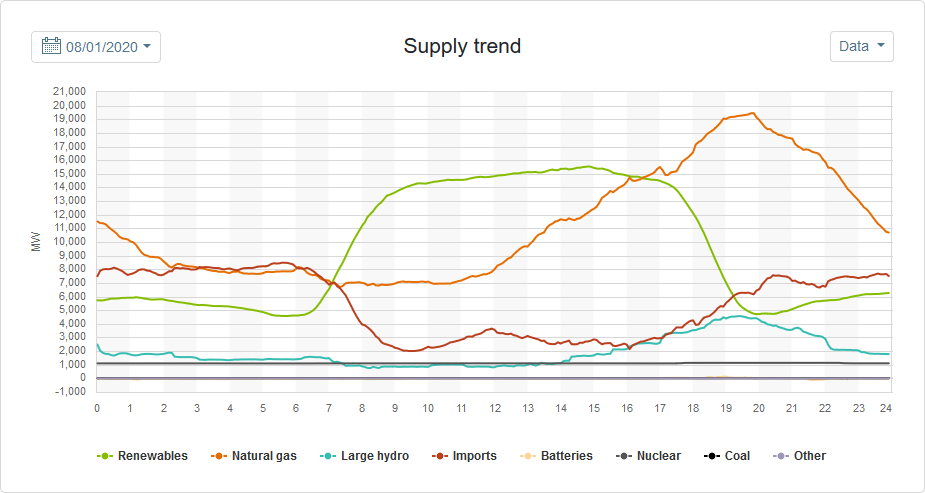
\includegraphics[width=0.9\linewidth]{california_supply_2020-08-01.png}
            \caption{Angebot an Energie in Kalifornien, USA, 01.08.2020
                \cite{Img_CaliforniaSupply}
            }
        \end{figure}
        \noindent
        Der tägliche Verbrauch erreicht vorallem um 17 Uhr bis 22 Uhr Höchstwerte.
        Nächte und Schlechtwettertage müssen dann durch gespeicherte, importierte
        oder lokale nicht-Solarenergie überbrückt werden, trotz der großartigen
        Vorraussetzungen für Solarenergie.
        \cite{SolarCalifornia, YouTube_RE-California}
        \begin{figure}[H]
            \centering
            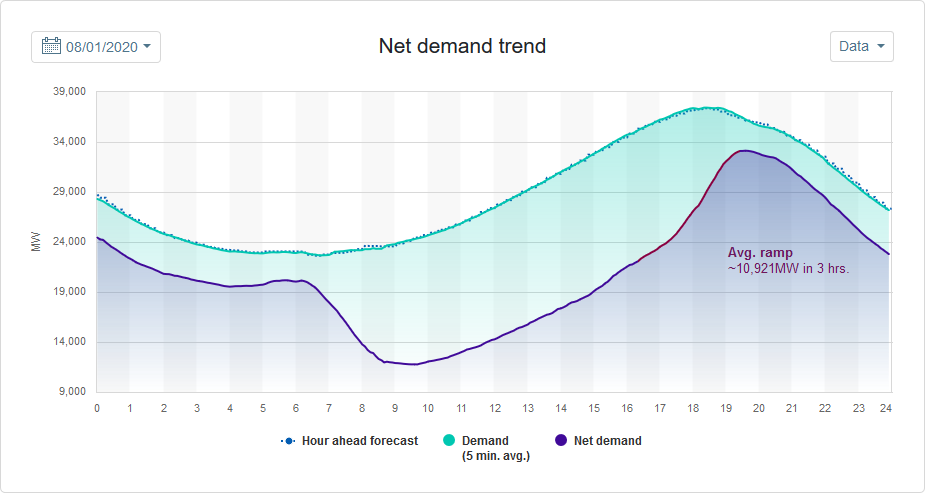
\includegraphics[width=0.9\linewidth]{california_demand_2020-08-01.png}
            \caption{Nachfrage an Energie in Kalifornien, USA, 01.08.2020
                \cite{Img_CaliforniaDemand}
            }
        \end{figure}